\documentclass{standalone}

\usepackage{pgfplots}
\usepackage{pgfplotstable}

\pgfplotsset{compat=newest}

\begin{document}

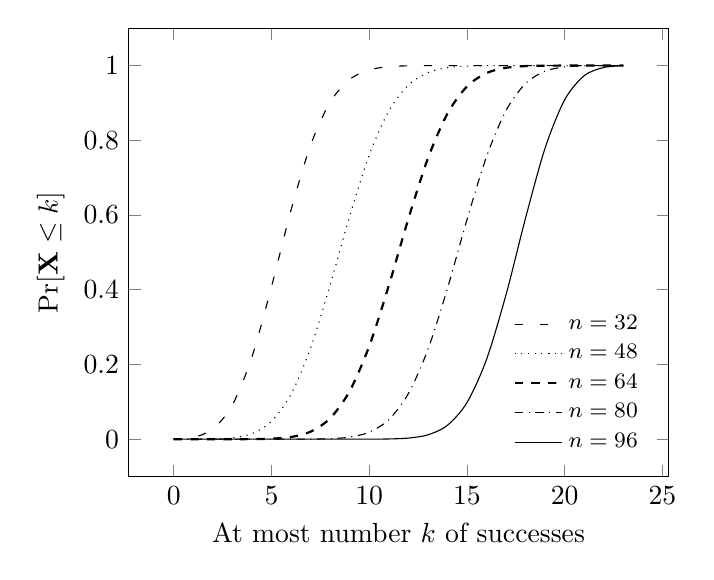
\begin{tikzpicture}[
  declare function = {
    binom(\n,\k) = \n! / (\k! * (\n - \k)!);
  },
  declare function = {
    hypergeom_dist_pmf(\N,\K,\n,\k)
      = binom(\K, \k) * binom(\N - \K, \n - \k) / binom(\N, \n);
  },
]
  \def\samples{24}
  \pgfplotstableset{
    create on use/x/.style = {
      create col/set list={0, ..., \samples}
    },
    create on use/y1/.style = {
      create col/expr accum = {
        \pgfmathaccuma + hypergeom_dist_pmf(128, \samples, 32, \pgfplotstablerow)
      }{0},
    },
    create on use/y2/.style = {
      create col/expr accum = {
        \pgfmathaccuma + hypergeom_dist_pmf(128, \samples, 48, \pgfplotstablerow)
      }{0},
    },
    create on use/y3/.style = {
      create col/expr accum = {
        \pgfmathaccuma + hypergeom_dist_pmf(128, \samples, 64, \pgfplotstablerow)
      }{0},
    },
    create on use/y4/.style = {
      create col/expr accum = {
        \pgfmathaccuma + hypergeom_dist_pmf(128, \samples, 80, \pgfplotstablerow)
      }{0},
    },
    create on use/y5/.style = {
      create col/expr accum = {
        \pgfmathaccuma + hypergeom_dist_pmf(128, \samples, 96, \pgfplotstablerow)
      }{0},
    },
  }

  \pgfplotstablenew[columns = {x, y1, y2, y3, y4, y5}]{\samples}{\loadedtable}

  \begin{axis}[
    smooth, legend pos = south east, ylabel = {$\Pr[\mathbf{X} \leq k]$},
    xlabel = {At most number $k$ of successes},
    legend style = { draw = none, font = \footnotesize, },
  ]
    \addplot+[black, loosely dashed, mark=none] table [y = y1] {\loadedtable};
    \addlegendentry{$n = 32$}

    \addplot+[black, dotted, mark=none] table [y = y2] {\loadedtable};
    \addlegendentry{$n = 48$}

    \addplot+[black, thick, dashed, mark=none] table [y = y3] {\loadedtable};
    \addlegendentry{$n = 64$}

    \addplot+[black, dashdotted, mark=none] table [y = y4] {\loadedtable};
    \addlegendentry{$n = 80$}

    \addplot+[black, solid, mark=none] table [y = y5] {\loadedtable};
    \addlegendentry{$n = 96$}
  \end{axis}
\end{tikzpicture}

\end{document}
